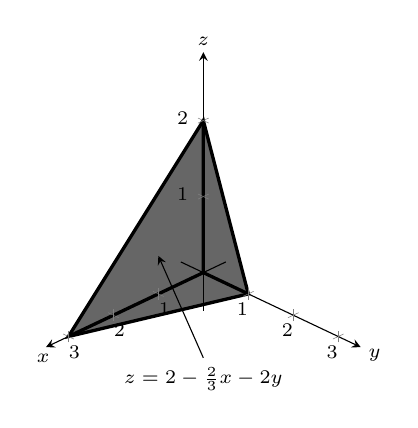
\begin{tikzpicture}[>=stealth]
\begin{axis}%
[width=175pt,height=200pt,
tick label style={font=\scriptsize},axis on top,
			axis lines=center,
			view={135}{25},
			name=myplot,
			xtick={1,2,3},
			ytick={1,2,3},
			ztick={1,2},
			%extra x ticks={1},
			%minor x tick num=1,
			%minor y tick num=4,
			%minor z tick num=1,
			%extra x tick labels={$a$},
			%extra y ticks={1},
			%extra y tick labels={$a$},
			%extra z ticks={1},
			%extra z tick labels={$h$},
			ymin=-.5,ymax=3.5,
			xmin=-.5,xmax=3.5,
			zmin=-.5, zmax=2.9,
			every axis x label/.style={at={(axis cs:\pgfkeysvalueof{/pgfplots/xmax},0,0)},xshift=-1pt,yshift=-4pt},
				xlabel={\scriptsize $x$},
			every axis y label/.style={at={(axis cs:0,\pgfkeysvalueof{/pgfplots/ymax},0)},xshift=5pt,yshift=-3pt},
				ylabel={\scriptsize $y$},
				every axis z label/.style={at={(axis cs:0,0,\pgfkeysvalueof{/pgfplots/zmax})},xshift=0pt,yshift=4pt},
				zlabel={\scriptsize $z$}
			]

\draw [{\colorone}, very thick] (axis cs: 3,0,0) -- (axis cs: 0,0,0)
																(axis cs: 0,1,0) -- (axis cs: 0,0,0)
																(axis cs: 0,0,2) --  (axis cs: 0,0,0);


\draw [{\coloronefill}, very thin,fill={\coloronefill},opacity=.6] (axis cs: 3,0,0) -- (axis cs: 0,1,0) -- (axis cs: 0,0,2) --  cycle;

\draw [{\colorone}, very thick] (axis cs: 3,0,0) -- (axis cs: 0,1,0) -- (axis cs: 0,0,2) --  cycle;

\draw [->] (axis cs: 2,2,0) node [below] {\scriptsize $z= 2-\frac23x-2y$} -- (axis cs: 1,0,.5);
%\draw [very thick,{\colorone},fill={\coloronefill}] (axis cs:0,0,0) -- (axis cs:0,4,0)-- (axis cs:2,4,0)-- (axis cs: 2,0,0) -- cycle;
%
%\draw [very thick,{\colorone},dashed] (axis cs:0,0,0) -- (axis cs:2,4,0);
%
%\draw (axis cs: 1,.5,0) node {\scriptsize $R_1$}
%(axis cs: 1,3.5,0) node {\scriptsize $R_2$};
%\addplot3[domain=-1:1,%y domain=0:1,surf,%fill=white,colormap={mp2}{\colormapplaneone},opacity=.6,faceted color=black!40,
%samples=21,samples y=0, thin, smooth,{\coloronefill},fill={\coloronefill}] ({x},{0},{6-2*x^2}) --cycle;
%
%\addplot3[domain=-1:1,%y domain=0:1,surf,%fill=white,colormap={mp2}{\colormapplaneone},opacity=.6,faceted color=black!40,
%samples=21,samples y=0, thin, smooth,{\coloronefill},fill={\coloronefill}] ({x},{0},{2+2*x^2}) --cycle;
%
%\addplot3[domain=-1:1,%y domain=0:1,surf,%fill=white,colormap={mp2}{\colormapplaneone},opacity=.6,faceted color=black!40,
%samples=21,samples y=0, thick, smooth,{\colorone}] ({x},{0},{6-2*x^2}) ;
%
%\addplot3[domain=-1:1,%y domain=0:1,surf,%fill=white,colormap={mp2}{\colormapplaneone},opacity=.6,faceted color=black!40,
%samples=21,samples y=0, thick, smooth,{\colorone}] ({x},{0},{2+2*x^2}) ;

%
%
%\addplot3[domain=-2:2,%y domain=0:1,surf,%fill=white,colormap={mp2}{\colormapplaneone},opacity=.6,faceted color=black!40,
%samples=21,samples y=0, thick, smooth,{\colorone},fill={\colortwofill}] ({0},{x},{4-x^2/2}) -- cycle;
%
%\draw (axis cs: 0,.5,3) node {\scriptsize $R_1$} 
			%(axis cs: 0,.5,5) node {\scriptsize $R_2$};
			%
%
%\draw [->] (axis cs: 0,-1.5,1.2) node [rotate=-10,below] {\scriptsize $z=4-y^2/2$} -- (axis cs:0,-1.5,2.8);
%
%\draw [->] (axis cs: 0,1.5,1.2) node [rotate=-10,below] {\scriptsize $z=6-y^2$} -- (axis cs:0,1.4,3.6);
%
%
%%\addplot3[domain=-2:2,%y domain=0:1,surf,%fill=white,colormap={mp2}{\colormapplaneone},opacity=.6,faceted color=black!40,
%samples=21,samples y=0, thick, smooth,{\colorone}] ({0},{x},{2});





\end{axis}


\end{tikzpicture}












